\documentclass[12pt,a4paper]{article}

% -------------------- Packages --------------------
\usepackage{graphicx}
\usepackage{float}
\usepackage{amsmath,amssymb,mathtools}
\usepackage{geometry}
\usepackage{xcolor}
\usepackage{booktabs}
\usepackage{caption}
\usepackage{array}
\usepackage{tabularx}
\usepackage{enumitem}
\usepackage{titlesec}
\usepackage{fancyhdr}
\usepackage{hyperref}
\usepackage[most]{tcolorbox}
\usepackage{fontspec}

% -------------------- Page Layout --------------------
\geometry{
	top=2.5cm,
	bottom=2.5cm,
	left=2.5cm,
	right=2.5cm
}

% -------------------- Fonts --------------------
\setmainfont{Times New Roman}

% -------------------- Spacing --------------------
\linespread{1.2}
\setlength{\parindent}{1.2em}
\setlength{\parskip}{0.35em}

% -------------------- Colors --------------------
\definecolor{mainblue}{RGB}{35, 70, 120}
\definecolor{softgray}{RGB}{245, 245, 245}

% -------------------- Section Styling --------------------
\titleformat{\section}
{\Large\bfseries\color{mainblue}}
{\thesection}
{0.8em}
{}

\titleformat{\subsection}
{\large\bfseries\color{mainblue}}
{\thesubsection}
{0.7em}
{}

\titlespacing*{\section}{0pt}{1.4em}{0.7em}
\titlespacing*{\subsection}{0pt}{1.1em}{0.5em}

% -------------------- Lists --------------------
\setlist[itemize]{
	topsep=0.3em,
	itemsep=0.25em,
	parsep=0pt,
	leftmargin=1.5em
}

\setlist[enumerate]{
	topsep=0.3em,
	itemsep=0.3em,
	parsep=0pt,
	leftmargin=1.5em
}

% -------------------- Captions --------------------
\captionsetup{
	font=small,
	labelfont=bf,
	justification=centering,
	skip=8pt
}

% -------------------- Tables --------------------
\renewcommand{\arraystretch}{1.25}
\newcolumntype{Y}{>{\centering\arraybackslash}X}

% -------------------- Header / Footer --------------------
\pagestyle{fancy}
\fancyhf{}
\fancyhead[R]{Project Report}
\fancyhead[L]{Ali Taghizadeh}
\fancyfoot[C]{\thepage}
\renewcommand{\headrulewidth}{0.4pt}

% -------------------- Hyperlinks --------------------
\hypersetup{
	colorlinks=true,
	linkcolor=mainblue,
	citecolor=mainblue,
	urlcolor=mainblue
}

\begin{document}
	
	\begin{titlepage}
		\centering
		\vspace*{1cm}
		
		{\Large\bfseries Amirkabir University of Technology (Tehran Polytechnic)\par}
		\vspace{0.4cm}
		{\large Computer Simulation Course\par}
		
		\vspace{2.5cm}
		
		{\large Project Report 2\par}
		\vspace{1cm}
		\rule{\linewidth}{0.4pt}\\[0.6cm]
		{\LARGE\bfseries Water Quality Analysis, Statistical Fitting,\\[0.3cm]
			Monte Carlo Simulation, and Importance Sampling\par}
		\rule{\linewidth}{0.4pt}
		
		\vspace{2.5cm}
		
		{\large
			
			\textbf{Ali Taghizadeh}\\[0.2cm]
			Student ID: 40313008\par}
		
		\vfill
		
		{\normalsize
			Project Repository:\\[0.2cm]
			\href{https://github.com/alitkbbl/Water-Quality-Rare-Events}{github.com/alitkbbl/Water-Quality-Rare-Events}\par}
		
		\vspace{1.2cm}
		
	\end{titlepage}
	
	
	
	\setcounter{page}{1}
	
	
	\section{Introduction and Problem Statement}
	
	In water quality monitoring systems, keeping chemical parameters within standard ranges is critically important for ensuring public health. Deviations of key variables, such as $pH$ or chemical concentrations, from permissible thresholds can lead to serious health risks. From a statistical perspective, since water treatment systems usually operate with high precision, the exceedance of these parameters beyond standard limits is very low-frequency and is classified as a \textbf{rare event (Rare Events)}.
	
	The main objective of this project is to mathematically model one of the water quality parameters and accurately estimate the probability of occurrence of these rare events in the distribution tails (Tail Distributions); that is, estimating a probability of the form
	\[
	\gamma = P(X > \tau)
	\]
	where $\tau$ is the critical threshold. Since for events with very low probability, for example $\gamma \approx 10^{-4}$, simple sampling methods (Standard Monte Carlo) suffer from high variance and severe computational cost, this project will, in later phases, move toward implementing advanced variance reduction techniques such as \textbf{importance sampling (Importance Sampling)}. The first step in this path is to understand the data accurately and find the best base probability distribution $f(x)$ for modeling, which is addressed in this section.
	
	
	\section*{Guide to the Analytical Questions}
	
	The answers to the four analytical questions of the project are provided in the following sections; the titles are clickable:
	
	\begin{itemize}[leftmargin=2em, itemsep=0.4em]
		\item \hyperref[sec:q1]{\textbf{Question 1:}} The effect of the covering constant $M$ on the acceptance rate and runtime of the accept-reject algorithm.
		\item \hyperref[sec:q2]{\textbf{Question 2:}} Analysis of weight stability and the role of the proposal distribution tail thickness.
		\item \hyperref[sec:q3]{\textbf{Question 3:}} The convergence rate of the standard Monte Carlo method and verification of the theoretical rate $\mathcal{O}(N^{-1/2})$.
		\item \hyperref[sec:q4]{\textbf{Question 4:}} Optimization of the shift parameter $\mu_q$ and possible reasons for the failure of importance sampling.
	\end{itemize}
	
	
	\section{Data Description and Statistical Analysis (Exploratory Data Analysis)}
	
	In the first step of the project, the water quality dataset \texttt{water\_potability.csv}, containing 3276 samples, was examined. Due to the presence of missing values (Missing Values) in parameters such as $pH$ and the need for a complete dataset for accurate distribution fitting, the parameter \textbf{chloramines (Chloramines)} was selected as the target variable. Chloramines is a continuous chemical parameter with no missing data, and its increase beyond the permissible limit is considered a public health risk and a rare event in this system.
	
	Statistical examinations show that the mean chloramines concentration in the data is $\mu \approx 7.12$ and its standard deviation is $\sigma \approx 1.58$. A very important point in the descriptive analysis of this variable is its skewness (Skewness), which was obtained to be approximately zero, namely $-0.012$. This value indicates the high symmetry of the data and its behavioral similarity to symmetric bell-shaped distributions. However, as observed in the box plot (Box-plot), outliers (Outliers) exist on both tails of the distribution, below 3 and above 11, which exactly form our critical regions for investigating rare events.
	
	\begin{figure}[H]
		\centering
		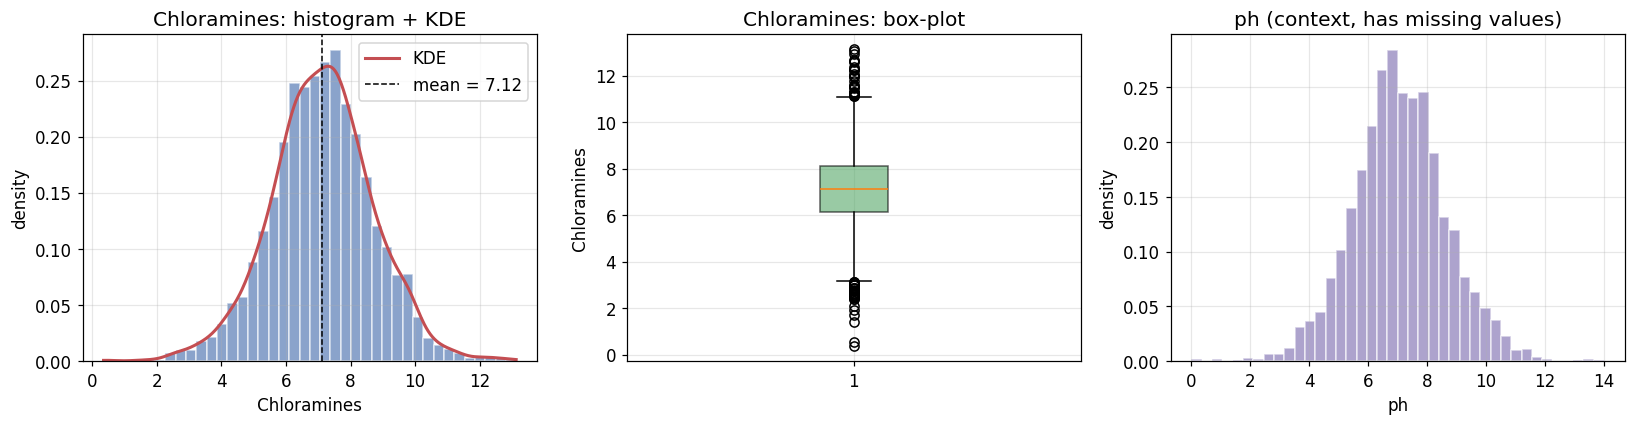
\includegraphics[width=0.95\textwidth]{../results/01_eda_overview.png}
		\caption{Frequency distribution and box plot of the chloramines variable. The overlap of the KDE curve with the histogram and the position of the mean line confirm the high symmetry of the data distribution.}
		\label{fig:eda-chloramines}
	\end{figure}
	
	\section{Mathematical Modeling and Distribution Fitting (Distribution Fitting)}
	
	To perform Monte Carlo simulations in the later phases, we need to find the best theoretical probability density function $f(x)$ that represents the behavior of the chloramines data. For this purpose, three distributions, \textbf{normal (Normal)}, \textbf{gamma (Gamma)}, and \textbf{Weibull (Weibull)}, were considered.
	
	To ensure the correctness of the calculations, the parameters of these distributions were estimated using two methods: a manual implementation of the \textbf{maximum likelihood estimation (Manual MLE)} algorithm and the use of optimized functions from the scipy library. The complete agreement between the outputs of these two methods, for example $\mu=7.1223$ and $\sigma=1.5828$ for the normal distribution in both cases, confirms the correctness of the algorithm implementations.
	
	To evaluate and select the best model, the log-likelihood criterion (Log-likelihood), Akaike information criterion (AIC), Bayesian information criterion (BIC), and the distance in the Kolmogorov-Smirnov test (KS) were used. The results are summarized in the table below:
	
	\begin{table}[H]
		\centering
		\caption{Comparison of fitting criteria for different distributions}
		\label{tab:distribution-fitting}
		\begin{tabularx}{\textwidth}{Y Y Y Y Y}
			\toprule
			\textbf{Distribution Model} & \textbf{Log-likelihood} & \textbf{AIC} & \textbf{BIC} & \textbf{KS Criterion} \\
			\midrule
			\textbf{Normal (Normal)} & \textbf{$-6152.856$} & \textbf{$12309.713$} & \textbf{$12321.902$} & \textbf{$0.021$} \\
			Weibull (Weibull) & $-6206.582$ & $12417.165$ & $12429.354$ & $0.039$ \\
			Gamma (Gamma) & $-6281.558$ & $12567.116$ & $12579.305$ & $0.047$ \\
			\bottomrule
		\end{tabularx}
	\end{table}
	
	\textbf{Analysis of the fitting results:}
	As is clear from the evaluation criteria, the \textbf{normal distribution} performs best by a meaningful margin. The lowest AIC and BIC values show that the normal distribution preserves the largest amount of information from the data with the least complexity. Also, the lowest KS error, namely $0.021$, indicates the highest agreement between the empirical cumulative distribution function (ECDF) and the theoretical model.
	
	The mathematical reason for this superiority goes back to the symmetric nature of the chloramines data, namely skewness close to zero; whereas gamma and Weibull distributions usually perform better for modeling skewed data (Skewed Data). The Q-Q plot also confirms this result; the empirical points lie well on the diagonal line, and only a very slight deviation is observed at the end of the extreme right tail (Extreme Right Tail), which is natural in limited sampling.
	
	\begin{figure}[H]
		\centering
		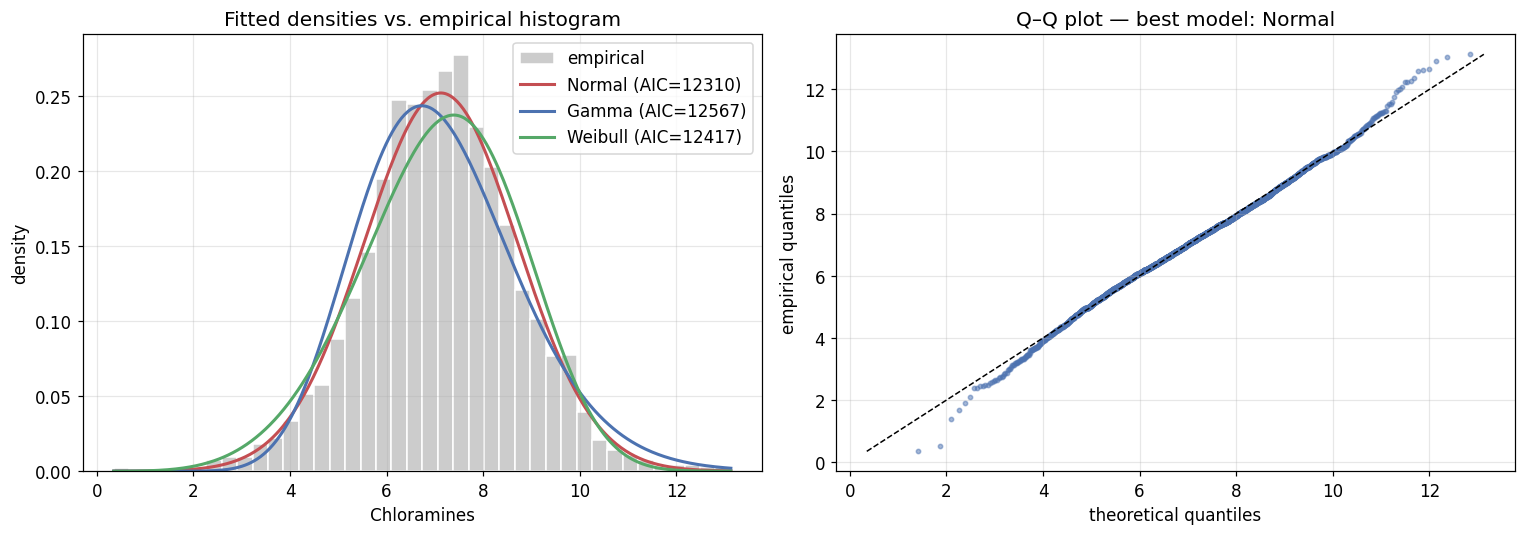
\includegraphics[width=0.95\textwidth]{../results/01_fit_comparison.png}
		\caption{Visual comparison of the fitted distribution functions on the empirical data on the left and the Q-Q plot for the normal model on the right. The visual error in the gamma and Weibull distributions is clearly evident around the peak of the distribution.}
		\label{fig:fitted-densities-qq}
	\end{figure}
	
	\section{Definition of the Rare-Event Threshold (Rare-Event Threshold)}
	
	Our final working model for the continuation of the project is the distribution $\operatorname{Normal}(\mu=7.1223, \sigma=1.5828)$. The goal of the simulation is to estimate the probability of critical chloramines values. To proceed with the computational phase, the critical threshold $\tau$ was set so that the probability of exceeding it under the theoretical model would be a rare event with probability exactly $\gamma = 10^{-4}$.
	
	Based on calculations of the survival function (Survival Function) on the normal model, this threshold was computed as \textbf{$\tau \approx 13.0089$}. Looking at the empirical data, it is observed that the maximum recorded value in the entire dataset is \textbf{$13.1270$}. This means that the threshold $\tau$ is located exactly at the far edge of the empirical distribution.
	
	From a simulation perspective, the rarity of this event is challenging; because if we want to estimate the probability of values greater than $13.0089$ with low error using crude Monte Carlo sampling (Standard MC), we will need millions of samples. This inefficiency will be demonstrated in the later notebooks and resolved using Importance Sampling.
	
	\section{Simulation and Synthetic Data Generation (Accept-Reject Sampling)}
	
	As mentioned earlier, analyzing rare events with probabilities such as $\gamma = 10^{-4}$ requires a huge amount of data. Since the real dataset contains only 3276 observations, in this phase of the project we must generate new samples using the fitted model, namely the normal distribution with $\mu=7.1223$ and $\sigma=1.5828$. Due to the restriction on using ready-made random number generation functions, such as \texttt{scipy.stats.norm.rvs}, the fundamental \textbf{accept-reject (Accept-Reject)} algorithm was implemented manually.
	
	\textbf{Algorithm design and proposal distribution selection:}
	In this method, the goal is to extract samples from the target distribution $f(x)$ using a simpler proposal distribution (Proposal Distribution) such as $g(x)$, provided that the following inequality always holds:
	\[
	f(x) \le M \cdot g(x)
	\]
	In this project, the proposal distribution was chosen as a \textbf{uniform (Uniform)} distribution over the interval $[a,b]$. Choosing this interval requires careful analysis:
	
	\begin{itemize}
		\item \textbf{Lower bound ($a = 0$):} Given the physical nature of the chloramines variable, namely chemical concentration, negative values are meaningless.
		\item \textbf{Upper bound ($b = \mu + 6\sigma \approx 16.62$):} In the normal distribution, the probability of data appearing beyond six standard deviations from the mean is less than $10^{-8}$. Therefore, truncating (Truncation) the distribution at this point introduces a completely negligible computational error.
	\end{itemize}
	
	By substituting the uniform distribution $g(x) = \frac{1}{b-a}$, the covering constant is computed as
	\[
	M = (b-a)\max f(x)
	\]
	whose value in this problem was obtained as \textbf{$M = 4.1891$}.
	
	\textbf{Validation (Validation) of the outputs:}
	Using this approach, 100,000 samples were generated. To verify the correctness of the generated samples, three criteria were considered:
	
	\begin{enumerate}
		\item \textbf{Moments:} The mean of the generated samples, namely $7.1221$, and their standard deviation, namely $1.5839$, are in almost perfect agreement with the theoretical parameters.
		\item \textbf{Statistical KS test:} The result of the Kolmogorov-Smirnov test with a p-value of $0.932$ shows that there is no statistical evidence to reject the hypothesis that the samples come from the distribution $f(x)$. In other words, the agreement is strong.
		\item \textbf{Visual inspection:} Comparing the histogram of the real data and the generated samples shows the degree of agreement of the algorithm.
	\end{enumerate}
	
	
	\begin{figure}[H]
		\centering
		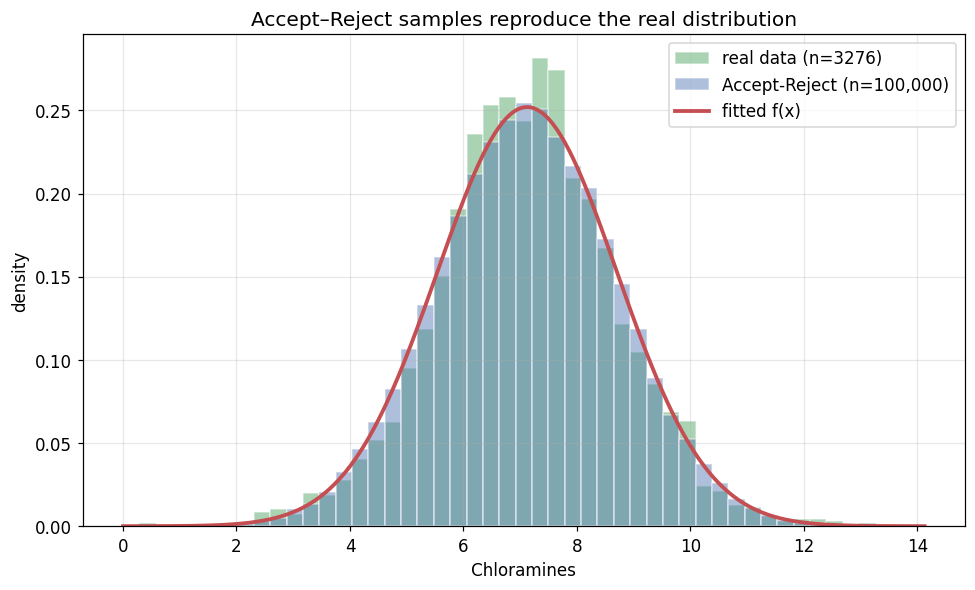
\includegraphics[width=0.95\textwidth]{../results/02_accept_reject_histograms.png}
		\caption{Comparison of the histogram of real data, samples simulated with the Accept-Reject method, and the density curve of the target distribution. The precise overlap of these three confirms the correct performance of the algorithm in reproducing the original distribution.}
		\label{fig:accept-reject-hist}
	\end{figure}
	
	\section{Efficiency Analysis: Investigating the Effect of the Covering Constant $M$ on Acceptance Rate and Runtime}
	
	\textbf{Answer to Analytical Question 1 (Analytical Question 1)}\label{sec:q1}
	
	The accept-reject algorithm, despite its simplicity and accuracy, can be highly inefficient from a computational perspective. The reason lies in the random variable $U$ and the following acceptance condition:
	\[
	U \le \frac{f(Y)}{M \cdot g(Y)}
	\]
	Mathematically, the expected value (Expected Value) of the acceptance rate in this algorithm is exactly equal to $\frac{1}{M}$. In other words, the larger the constant $M$ is, the larger the dead space (Dead Space) between the envelope distribution and the target distribution becomes, and more samples are wasted or rejected.
	
	To investigate this phenomenon empirically, the algorithm was run with different widths for the uniform proposal distribution, from a radius of $3\sigma$ to $20\sigma$. The results obtained in the following table and plots contain two key analyses:
	
	\begin{figure}[H]
		\centering
		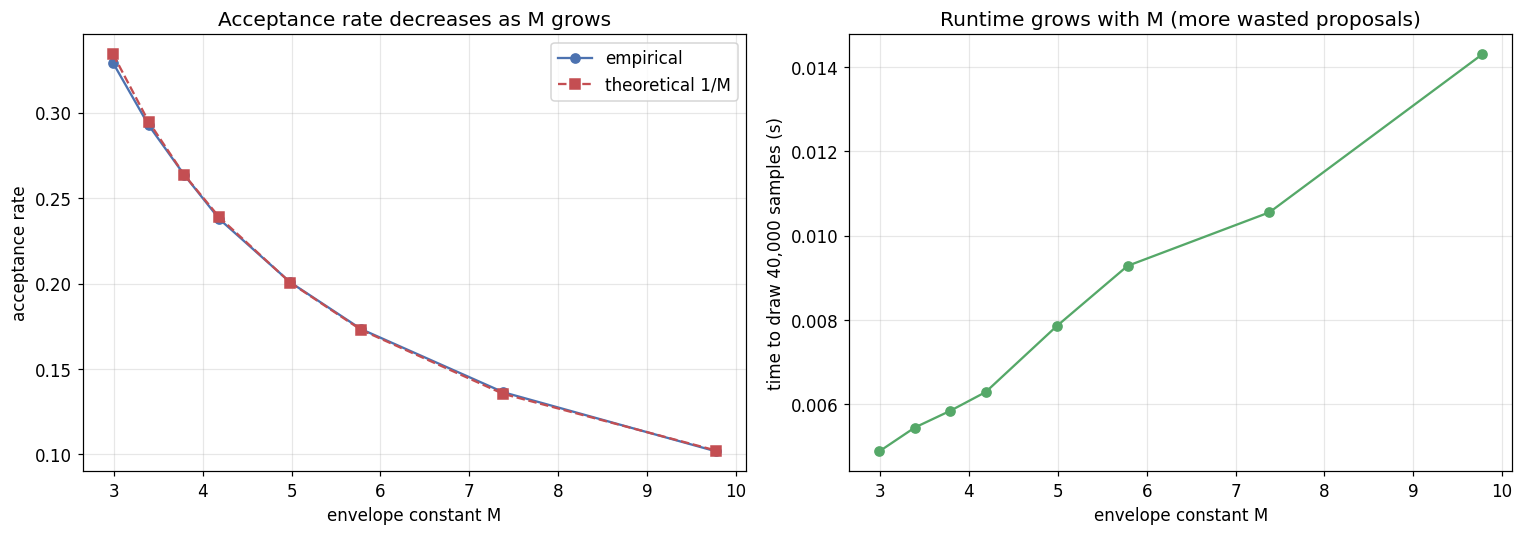
\includegraphics[width=0.95\textwidth]{../results/02_acceptance_vs_M.png}
		\caption{Left: decrease in acceptance rate with increasing constant $M$ and precise agreement of empirical behavior with the theoretical formula $1/M$. Right: linear increase in runtime along with the increase in wasted samples.}
		\label{fig:acceptance-rate-runtime}
	\end{figure}
	
	\textbf{Acceptance rate analysis (Acceptance Rate):}
	As observed in the table and the left plot, in the most optimal case, namely $M=2.9921$, only about $33\%$ of samples are accepted. By widening the bounds and reaching $M \approx 9.77$, the acceptance rate drops to about $10.2\%$. The complete agreement between the empirical blue points and the theoretical red points in the plot indicates completely random and independent behavior in the implemented algorithm. In our working model, namely $M=4.1891$, the acceptance rate is about $23.8\%$; this means that to generate 100 thousand valid data points, the algorithm had to generate and process more than 420 thousand proposal samples, equivalent to $76\%$ computational waste.
	
	\textbf{Runtime complexity analysis (Runtime Complexity):}
	The right plot shows the direct relationship between increasing $M$ and the runtime of the algorithm. From the perspective of computational complexity, to extract $N$ successful samples, the algorithm loop must be repeated on average $N \times M$ times. Therefore, the runtime is of order $\mathcal{O}(M)$ and has an increasing trend.
	
	\textit{Analytical note:} Minor fluctuations and ups and downs in the runtime plot, for example the decrease in time around $M \approx 3.5$, are a common phenomenon in micro-level evaluations (Micro-benchmarking). Since times are recorded on the scale of thousandths of a second, namely milliseconds, these fluctuations are caused by operating system scheduling (OS Scheduling), CPU cache state (CPU Cache), and background processes (Background Processes); however, the overall macro-trend (Macro-trend) is clearly increasing and consistent with the mathematical analysis of the algorithm.
	
	\textbf{Conclusion for entering the next phase:}
	The accept-reject algorithm was successful for generating general data, but it showed that due to its sample rejection nature, it is costly. Now, if we want to estimate a rare event with probability $10^{-4}$, such as chloramines exceeding the threshold $\tau=13.0089$, using only these generated data, namely the standard Monte Carlo method, we need to generate millions of samples. Considering the $76$ percent waste of this algorithm, we will face a severe computational bottleneck. This is exactly the reason that necessitates more advanced methods such as Importance Sampling.
	
	\section{Standard Monte Carlo Estimation (Standard Monte Carlo) and the Challenges of Rare Events}
	
	After modeling the data, namely $\mu=7.1223$ and $\sigma=1.5828$, and determining the risk threshold, namely $\tau=13.0089$, the main goal of the project is to estimate the probability of occurrence of the rare event
	\[
	\gamma = P(X > \tau)
	\]
	whose true value is equal to $10^{-4}$.
	
	The most natural and simplest approach for this task is to use the standard Monte Carlo method (Crude Monte Carlo). In this method, $N$ independent samples $X_1,\dots,X_N$ are generated from the target distribution $f(x)$ using the Box-Muller algorithm, and the probability $\gamma$ is estimated by averaging the indicator function (Indicator Function):
	\[
	\hat{\gamma}_{MC} =
	\frac{1}{N}
	\sum_{i=1}^{N}
	\mathbb{I}(X_i > \tau)
	\]
	
	Mathematically, this estimator is \textbf{unbiased (Unbiased)}, because:
	\[
	\mathbb{E}[\hat{\gamma}_{MC}] = \gamma
	\]
	However, when facing rare events, the main issue is not unbiasedness, but the \textbf{variance (Variance)} of the estimator.
	
	\subsection{Comprehensive Evaluation of the Performance and Limitations of Standard Monte Carlo}
	
	In the standard Monte Carlo (SMC) method, since each event is a Bernoulli variable with success probability $\gamma$, the variance of the estimator $\hat{\gamma}_{MC}$ is:
	\[
	\operatorname{Var}(\hat{\gamma}_{MC}) = \frac{\gamma(1-\gamma)}{N}
	\]
	But in the evaluation of rare events, the criterion of vital importance is the \textbf{relative error (Relative Error)}, which is defined as the coefficient of variation (Coefficient of Variation):
	\[
	\text{Relative Error} =
	\frac{\sqrt{\operatorname{Var}(\hat{\gamma}_{MC})}}{\gamma} =
	\sqrt{\frac{1-\gamma}{N\gamma}} \approx \frac{1}{\sqrt{N\gamma}}
	\]
	This mathematical relationship reveals the core challenge in estimating rare events with the Monte Carlo method. The simulation results presented in the table depict exactly this crisis:
	
	\begin{itemize}
		\item \textbf{At $N = 10^3$ (sampling disaster):} The denominator of the relative error fraction is $\sqrt{1000 \times 10^{-4}} = \sqrt{0.1} \approx 0.316$, which leads to a crushing relative error of about $3.16$. More importantly, in \textbf{$92.6\%$} of the runs, the estimator returns exactly \textbf{zero}. This phenomenon, called the Zero-Estimate Phenomenon, can be explained using the Poisson approximation: the expected number of events is $N\gamma = 0.1$; according to the Poisson distribution, the probability of observing zero events is $e^{-0.1} \approx 0.904$, which agrees with the empirical result. A zero estimate in reliability engineering means that failure is impossible, which is a completely misleading and dangerous conclusion.
		\item \textbf{At $N = 10^4$:} Still, in $35.5\%$ of experiments, no rare event is observed, and the relative error $1.00$ equivalent to $100\%$ indicates severe uncertainty.
		\item \textbf{Stability at $N \ge 10^5$:} Only when the sample size reaches hundreds of thousands to one million, i.e., $N\gamma \gg 1$, does the estimator become stable and the relative error decrease below $10\%$.
	\end{itemize}
	
	These behaviors are visually shown in Figure~\ref{fig:mc-evaluation-combined}.
	
	\begin{figure}[H]
		\centering
		
		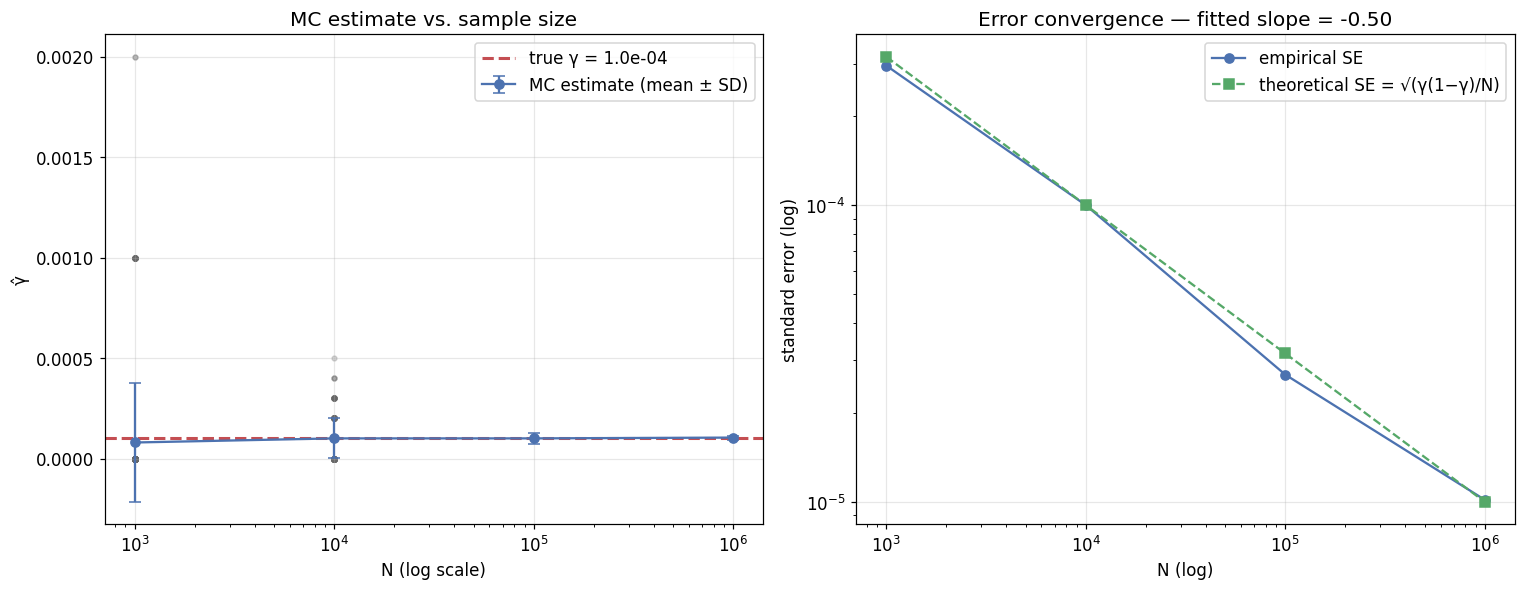
\includegraphics[width=0.95\textwidth]{../results/03_mc_convergence.png} 
		\caption{Evaluation of the performance and convergence of the standard Monte Carlo method. \textbf{Left plot:} shows the severity of dispersion and uncertainty of the estimator at different sample sizes. At $N=10^3$, the confidence intervals are very large, but as $N$ increases, the estimates converge around the true value, shown by the red dashed line. \textbf{Right plot:} convergence of the standard error on the Log-Log scale. The empirical slope ($ -0.50$) is in complete agreement with the theoretical convergence rate ($\mathcal{O}(N^{-1/2})$) and confirms the correctness of the simulation.}
		\label{fig:mc-evaluation-combined}
	\end{figure}
	
	\subsubsection*{Analysis of the Convergence Rate and Verification of Theory (Answer to Analytical Question 3)}\label{sec:q3}
	
	The key question is: at what rate does the Monte Carlo method converge, and can this convergence be accelerated? The right plot in Figure~\ref{fig:mc-evaluation-combined} answers this question. According to theory, the standard error (SE) is proportional to $N^{-1/2}$:
	\[
	\log(\text{SE}) \approx \log(\sqrt{\gamma}) - \frac{1}{2}\log(N)
	\]
	This equation predicts a straight line with a \textbf{slope exactly equal to $-0.5$} in the Log-Log plot. As shown in the plot title and the notebook calculations, the fitted empirical slope is \textbf{$-0.50$}, which confirms the theory with very high accuracy.
	
	\textbf{Engineering interpretation of this slope:} This slope represents the curse of Monte Carlo (Curse of Monte Carlo). This rate shows that computational error decreases with the square root of the sample size. In simpler terms:
	\begin{itemize}
		\item To \textbf{halve} the error, we must \textbf{quadruple} the computational volume.
		\item To add \textbf{one decimal digit of accuracy}, a 10-fold reduction in error, we must increase the computational volume by \textbf{100 times}.
	\end{itemize}
	
	\textbf{Conclusion for entering the final phase:} The analysis of this section proved that although standard Monte Carlo is theoretically correct and unbiased, it is highly inefficient for events with probability $10^{-4}$ and lower. The problem is not the slope $ -0.5$, but the large proportionality constant in the relative error relationship, $1/\sqrt{\gamma}$. This inefficiency is the main motivation for using the \textbf{importance sampling (Importance Sampling)} method in the next section; a method that aims to strongly reduce this constant and provide a stable estimate with a much smaller sample size.
	
	
	\section{Importance Sampling (Importance Sampling) and Breaking the Variance Barrier}
	
	As observed in the previous section, the standard Monte Carlo method (Crude MC) wastes most of its computational power in the main body of the distribution, where the indicator function $\mathbb{I}(X > \tau) = 0$. To solve this problem, we use the \textbf{importance sampling (IS)} technique. The main idea of this method is rooted in the mathematical concept of change of measure (Change of Measure).
	
	Instead of generating samples from the original distribution $f(x)$, we generate them from a proposal distribution $q(x)$ whose center of mass has been shifted toward the rare-event region, namely the threshold $\tau$. To preserve the unbiasedness property of the estimator, each sample is corrected with an importance weight (Importance Weight) equal to $w(x) = f(x)/q(x)$:
	\[
	\gamma =
	\mathbb{E}_f[\mathbb{I}(X>\tau)]
	=
	\mathbb{E}_q
	\left[
	\mathbb{I}(X>\tau)
	\frac{f(X)}{q(X)}
	\right]
	\]
	\[
	\hat{\gamma}_{IS} =
	\frac{1}{N}
	\sum_{i=1}^{N}
	\mathbb{I}(X_i > \tau) w(X_i),
	\qquad
	X_i \sim q
	\]
	
	\textbf{Design of the proposal distribution:}
	In this model, $q(x)$ was chosen as a normal distribution whose mean is set exactly on the risk threshold, namely $\mu_q = \tau = 13.0089$, and whose standard deviation is equal to that of the original distribution, namely $\sigma_q = 1.5828$. This shift causes approximately half of the generated samples to lie in the critical region, namely $X > \tau$.
	
	\textbf{Remarkable variance reduction results:}
	The simulation output tables prove the outstanding power of this method:
	
	\begin{itemize}
		\item \textbf{Solving the zero-estimate problem:} At sample size $N=10^4$, while the MC method recorded no event in $35.5\%$ of cases, i.e., $\hat{\gamma} = 0$, the IS method reduced the zero-estimate rate to \textbf{$0\%$} because of direct sampling from the critical region.
		\item \textbf{Variance reduction factor (Variance Reduction Factor):} The variance of the IS estimator is between \textbf{$2256$ and $3202$ times} lower than that of MC.
		\item \textbf{Reduction of relative error:} At $N=10^4$, the relative error decreased from $102.6\%$ in the MC method to only \textbf{$2.0\%$} in the IS method. In other words, the accuracy of the IS method with $10^4$ samples is equivalent to the accuracy of the MC method with more than $25 \times 10^6$ samples.
	\end{itemize}
	
	\subsection{Visual Analysis of Importance Sampling Performance Compared with Monte Carlo}
	
	For a more accurate evaluation and intuitive understanding of the superiority of IS, a three-part plot has been drawn that compares three key aspects:
	
	\begin{figure}[H]
		\centering
		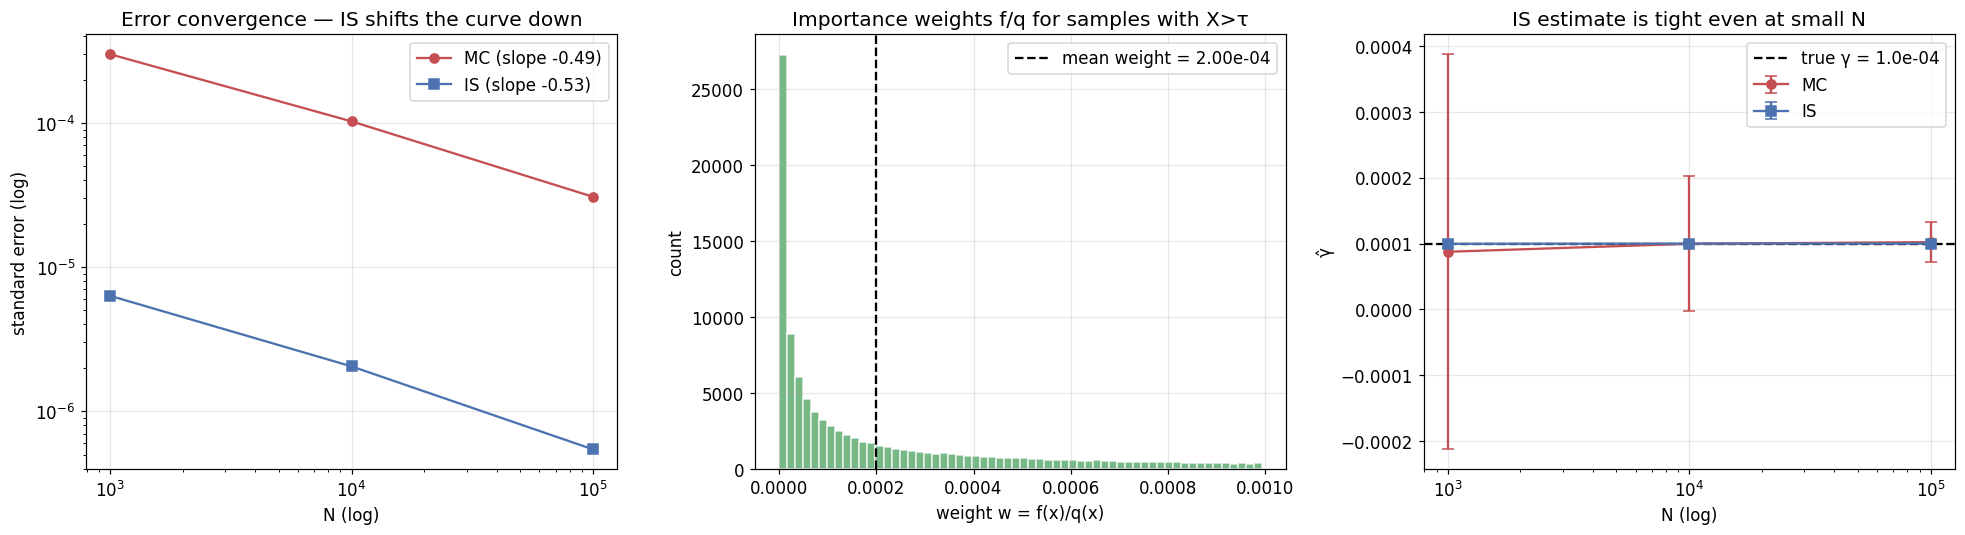
\includegraphics[width=0.95\textwidth]{../results/04_importance_sampling.png}
		\caption{Three-way comparison of Importance Sampling and Monte Carlo performance: error convergence, histogram of weights, and estimate stability at different sample sizes.}
		\label{fig:is-vs-mc-triple}
	\end{figure}
	
	\begin{enumerate}
		\item \textbf{Error convergence:} The Log-Log plot of the standard error shows that both methods follow the theoretical convergence rate $\mathcal{O}(N^{-1/2})$; the slope is $-0.49$ for MC and $-0.53$ for IS. However, shifting the distribution has reduced the error of the IS method by about two to three orders of magnitude (Order of Magnitude) compared with MC.
		\item \textbf{Distribution of importance weights:} This histogram shows the stability of the weights in the rare region. The weights have very small values, with an average of approximately $2.00 \times 10^{-4}$, and there is no single abnormal-weight sample that would disrupt the averaging process.
		\item \textbf{Estimate stability at low sample size:} This plot illustrates the failure of MC when facing a rare event; at $N=10^3$, the MC error bars are so large that they reach negative values. In contrast, the IS estimate, even at this small sample size, matches the true probability, namely $\gamma = 1.0 \times 10^{-4}$, with high accuracy and very narrow error bars.
	\end{enumerate}
	
	\section{Analysis of Weight Stability and Distribution Tail Thickness}
	
	\textbf{Answer to Analytical Question 2}\label{sec:q2}
	
	As observed in the middle plot of the previous section, weight stability is the key to the success of IS. One of the hidden risks in this method is the phenomenon of \textbf{variance explosion (Variance Explosion)} due to unstable weights.
	
	\textbf{The golden rule in IS:}
	\textit{The proposal distribution $q(x)$ must have a heavier tail (Heavier Tail), or at least a tail equal to that of the target distribution $f(x)$, in the region of interest.}
	
	The mathematical reason for this lies in the ratio $w(x) = \frac{f(x)}{q(x)}$. If $q(x)$ has a lighter tail than $f(x)$, for example $\sigma_q = 0.5\sigma$, then as we move toward infinity, the denominator of the fraction approaches zero much faster than the numerator, and as a result:
	\[
	\lim_{x \to \infty} w(x) = \infty
	\]
	This means that if, by chance, a sample is generated at the far end of the tail, it receives an astronomical weight that disrupts the entire average and explodes the variance.
	
	To quantify this stability, the criterion \textbf{effective sample size (Effective Sample Size - ESS)} is used:
	\[
	ESS =
	\frac{\left(\sum w_i\right)^2}{\sum w_i^2}
	\]
	If the weights are uniform, $ESS \approx N$, and if one sample receives an infinite weight, $ESS \to 1$.
	
As clearly illustrated in Figure \ref{fig:weight-tails-analysis}, selecting a proposal distribution with lighter tails (red curve) causes the importance weight function to grow exponentially, driving the logarithm of the weights to astronomically large values (up to the order of $10^{60}$). This behavior directly leads to the divergence of the second moment and, consequently, an infinite estimator variance. In contrast, the heavier-tailed proposal distribution (green curve) exhibits a well-bounded and stable behavior throughout the domain.

\begin{figure}[H]
	\centering
	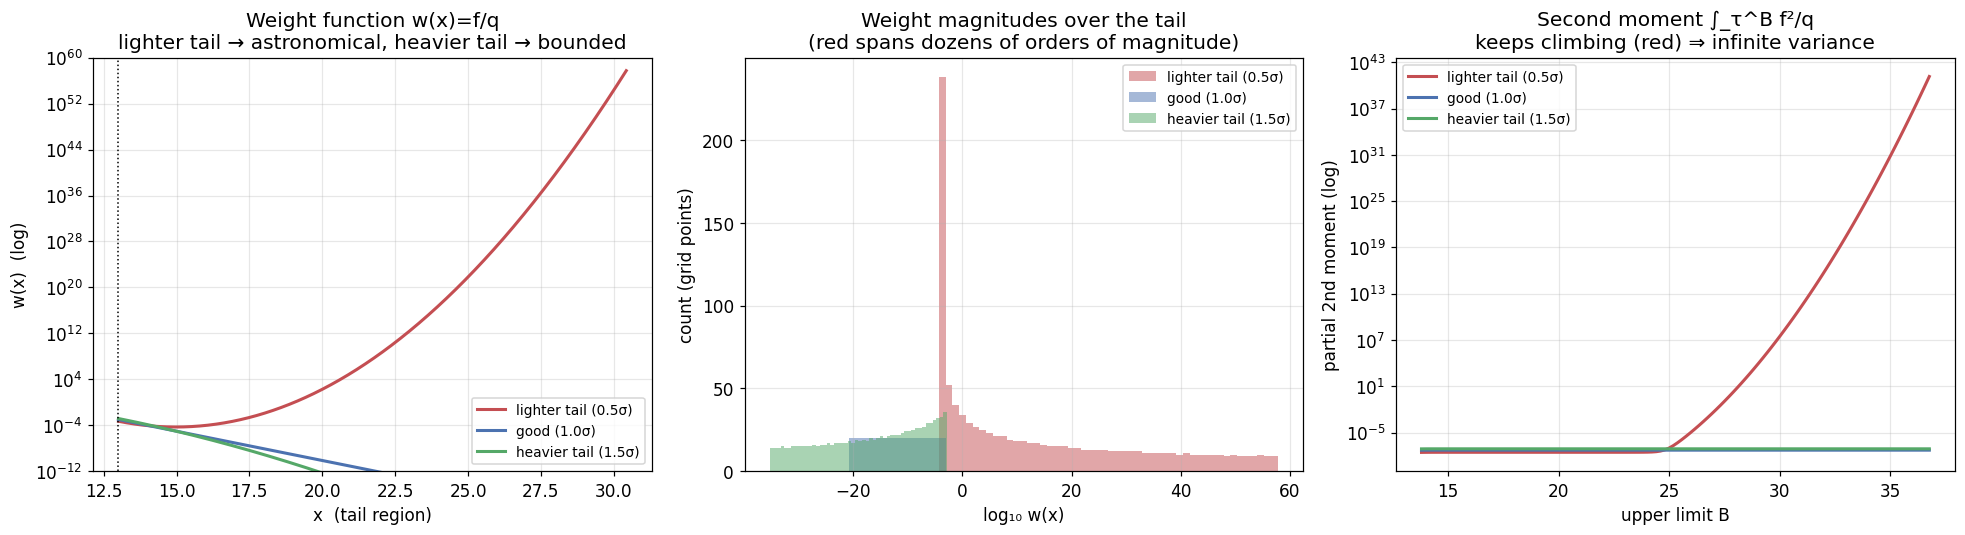
\includegraphics[width=0.95\textwidth]{../results/04_weight_tails_Q2.png}
	\caption{Impact of proposal-tail thickness on importance sampling. From left to right: exponential growth of the importance weight function under a lighter-tailed proposal, the enormous spread in the histogram of log-weights, and the increasing second moment indicating variance explosion. These behaviors are contrasted with the bounded and stable performance obtained using a heavier-tailed proposal distribution.}
	\label{fig:weight-tails-analysis}
\end{figure}

The practical consequences of this structural difference are also clearly reflected in the Effective Sample Size (ESS). In the lighter-tailed case ($\sigma_q = 0.5\sigma$), a small number of samples with extremely large weights dominate the estimator, as evidenced by the weight histogram. As a result, the ESS collapses dramatically, yielding an $\mathrm{ESS}/N$ ratio of only $0.0002$, which indicates severe estimator instability and an effective breakdown of the sampling procedure. By contrast, in the heavier-tailed case ($\sigma_q = 1.5\sigma$), the proposal density $q(x)$ remains sufficiently large in the tails, preventing the importance weights from becoming excessively large. Consequently, the weights remain well-behaved and the $\mathrm{ESS}/N$ ratio improves substantially to $0.0170$. Together, these quantitative results and visual observations confirm a fundamental principle of importance sampling: \textbf{to ensure stability and avoid variance explosion, the proposal distribution should possess tails at least as heavy as, and preferably heavier than, those of the target distribution.}

	
	\section{Optimization of the Shift Parameter and Reasons for IS Failure}
	
	\textbf{Answer to Analytical Question 4}\label{sec:q4}
	
	Is success always guaranteed in the IS method? No. A poor choice of the mean of the proposal distribution, namely $\mu_q$, can make IS perform even worse than standard Monte Carlo.
	
	To understand this, the relative error of the IS method for different values of $\mu_q$ has been plotted in a graph that shows a \textbf{U-shaped (U-shaped)} curve:
	
	\begin{enumerate}
		\item \textbf{Insufficient shifting (Under-shifting), $\mu_q \approx \mu$:} If $\mu_q$ remains close to the original mean, namely $7.12$, the proposal distribution is not significantly different from the original distribution. In this case, most samples still fall outside the rare region, and due to the noise caused by multiplication by the weights, the variance of the estimator may even become slightly higher than standard MC.
		\item \textbf{Excessive shifting (Over-shifting), $\mu_q \gg \tau$:} If we move the distribution too far forward, for example $\mu_q = 19$, almost all samples become greater than $\tau$, but because they are very far from the body of $f(x)$, their weights, namely $f(x)/q(x)$, tend strongly toward zero. Meanwhile, the few samples that fall on the left side of this distribution and close to $\tau$ will have relatively very large weights. This severe asymmetry causes a sharp drop in ESS and a significant increase in relative error on the right side of the U-shaped plot.
		\item \textbf{Optimal point (Sweet Spot):} The best performance occurs exactly near the threshold $\tau$. Here, $\mu_q \approx 14.25$ records the best result with a relative error of $0.014$. In this region, both the number of successful samples is high and the weight distribution is balanced and stable.
	\end{enumerate}
	
	\begin{figure}[H]
		\centering
		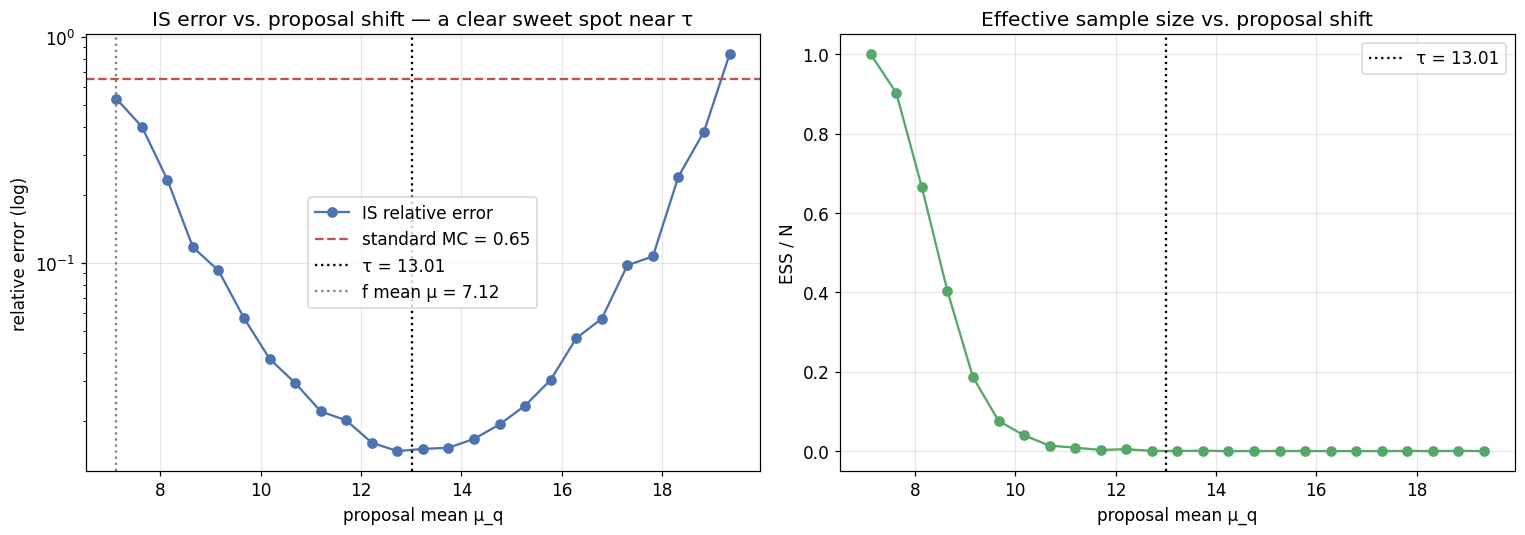
\includegraphics[width=0.95\textwidth]{../results/04_proposal_shift_Q4.png}
		\caption{U-shaped behavior of the IS error with respect to mean shifting on the left, and the sharp drop in effective sample size when moving away from the optimal point on the right.}
		\label{fig:is-error-proposal-shift}
	\end{figure}
	
	\section{Final Summary and Conclusion of the Project}
	
	This project successfully followed a complete engineering and statistical path for evaluating rare events in water quality, focusing on the Chloramines variable:
	
	\begin{enumerate}
		\item \textbf{Statistical modeling:} Initially, using MLE fitting, the normal distribution was identified as the best model describing the data, and the probability of the critical threshold $\tau = 13.0089$ was determined to be the rare value $10^{-4}$.
		\item \textbf{Basic random generation:} The Accept-Reject algorithm was implemented fundamentally. Although this method was successful for generating data consistent with the distribution, it showed that it is highly inefficient for exploring the distribution tail.
		\item \textbf{The standard Monte Carlo challenge:} The simulation showed that the Crude MC method suffers from the zero-estimate phenomenon and requires millions of samples to reach an acceptable error; this proved its slow convergence rate $\mathcal{O}(N^{-1/2})$ and high variance.
		\item \textbf{Advanced variance reduction technique:} Finally, using the importance sampling algorithm (Importance Sampling), a paradigm shift was made from increasing sample size to intelligently changing the distribution. By carefully choosing $\mu_q \approx \tau$ and satisfying the tail-thickness condition of the proposal distribution, the variance of the problem was reduced by more than $2500$ times, and accurate estimation of the rare event became possible with a very small computational volume.
	\end{enumerate}
	
	This analytical framework shows that in risk management and reliability, using advanced stochastic simulation methods is not a choice, but a computational necessity.
	
\end{document}
